\chapter{Link Modelling}\label{ch:linkmodel}
The goal of this chapter is to be able to estimate the probability, based on the topology of a wireless network, of how likely it is that packet loss will happen during a transmission between two nodes.

This chapter...\medbreak

\begin{figure}[ht]
    \centering
    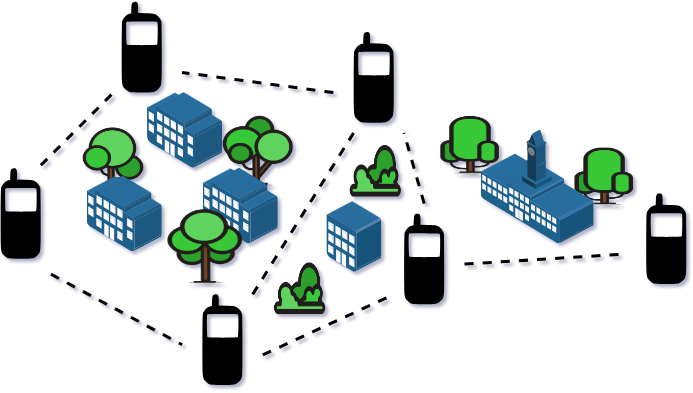
\includegraphics[width=.7\textwidth]{figures/manet_with_terrain.png}
    \caption{A sample wireless network topology.}
    \label{figure:manetwithter}
\end{figure}

\autoref{figure:manetwithter} shows a sample wireless network topology for a \acrfull{manet}. The network consists of mobile devices (nodes), and the communication between these (links). Nodes are \doublequote{linked} with other nodes when they are able to communicate wirelessly. Wireless communication relies on the transmission and reception of electromagnetic waves~\cite[p.~10]{paper:linkmodel} (radio signals), and the strength, or quality, of a wireless link is described by the signal loss occurring when propagating the signal from transmitter to receiver. In \cite{paper:linkmodel}, the term \gls{pathloss} is used to describe this signal loss, and is determined in part by the physical distance between transmitter and receiver, but also by physical objects and terrain, like buildings or forests. \autoref{sec:linkmodel} will elaborate further on the \gls{pathloss} of a link, as well as present a method for simulating the \gls{pathloss} for a mobile network topology. Another major consideration for mobile networks is that the topology is dynamic. Nodes move around, causing existing links to disappear, or new links to appear, thus changing the topology of the network.

%Whether nodes are able to communicate wirelessly with each other depends on the \gls{pathloss} 

%In \autoref{figure:manetwithter} we see a topology of six nodes, with seven communication links between them.
%When working with wireless mobile networks, it is important keep in mind that the topology these networks are dynamic. Nodes move, causing the topology to change. When nodes move in or out of reach of other nodes, links will appear or disappear dynamically.

%to keep two things in mind: First, the topology a mobile network is, per definition, dynamic.

\section{Link Modelling}\label{sec:linkmodel}

In this section, we will present a method for simulating \gls{manet} link \gls{pathloss} from \cite{paper:linkmodel}. For our simulations, we would like to be able to simulate the performance of a \gls{manet}. The performance is, however, heavily dependent on network conditions and the capabilities of the technology~\cite[p.~10]{paper:linkmodel}. The author of \cite{paper:linkmodel} presents methods for evaluating the performance of a wireless networks, and proceeds to introduce methods for simulating \gls{pathloss} on a multi-link model, based on a real-world performance measurement. \autoref{sec:pathloss} will summarise the method for simulating \gls{pathloss} on a \gls{manet}, and \autoref{sec:simulatingvalues}...
Note that the actual values used in this Section, is specific to the Reachi\todo[inline]{Introduce Reachi earlier in the report.} devices, and are based on on-site measurements.

\subsection{Units}
In the following sections, we will be using different units of measurements. For distances, all measurements (e.g., the distance between two nodes) will be in meters. We describe the strength of a radio signal using \acrfull{db}~\cite{website:isadbdbm}, and the transmission power as \acrfull{dbm}~\cite{website:isadbdbm}.

\subsection{Path Loss}\label{sec:pathloss}
The \gls{pathloss} of a link is dependent on the distance between transmitter and receiver, as well as a stochastic shadow fading term. The \gls{pathloss} vector \vect{PL_{db}} is the sum of two parts:

%\vect{l_{pl}} = \vect{l_d} + \vect{l_{fading}}

\begin{description}
    \item[\vect{PL_{determ,dB}(d)}]: A deterministic distance dependent part, which describes the mean signal attenuation at any given link distance (distance between transmitter and receiver), in \gls{db}. It is a vector of size $n$, where $n$ is the number of links in the network.
    \item[\vect{PL_{fading,dB}}]: A stochastic slow/shadow fading part, which specifies the local mean of the signal, in \gls{db}. The slow fading variable is, more or less, constant in the same local area, as it is caused by terrain, buildings, vegetation, and cars. It is a vector of size $n$, where $n$ is the number of links in the network.
\end{description}
\begin{eq}\label{eq:pathlossdb}
    \vect{PL_{dB}} = \vect{PL_{determ,dB}(d)} + \vect{PL_{fading,dB}}
\end{eq}

The deterministic distance dependent \gls{pathloss} is an independent value, while the stochastic slow/shadow fading value depends on physical objects and terrain. This means that links existing in the same physical environment should have a similar slow fading. The similarity is modelled by introducing a correlation between the slow fading on different links:

\begin{description}
    \item[Cross correlation (interlink)] describes the correlation between two or more links in the same spatial (physical) environment (\textbf{spatial correlation}).
    \item[Auto correlation (intralink)] describes the correlation in the development of slow fading for a single link over time (\textbf{temporal correlation}).
\end{description}

The \gls{pathloss} can be used, along with the transmission power in \acrshort{dbm} ($P_{tx,dBm}$) to simulate the \gls{rssi} on a link.
%\begin{eq}\label{eq:computerssi}
%    RSSI_{dBm} = P_{tx,dBm} - PL_{dB}
%\end{eq}

\begin{eq}\label{eq:pathlosslink}
    \vect{l_{pl}} = \vect{l_d} + \vect{l_{fading}}
\end{eq}

\todo[inline]{use the same notation everywhere}

\subsection{Simulating Link Path Loss}\label{sec:simulatingvalues}
In this Section, we will summarise how \gls{pathloss} and \gls{rssi} values are simulated for a \gls{manet} according to \cite{paper:linkmodel}, and we will present how we expect to use this in our own simulations. Again, note that the values used throughout this section are based on on-site measurements made with the Reachi devices in the Philippines and are heavily dependent on the environment, as described in \cite{paper:linkmodel}. \medbreak

%With a \gls{manet} consisting of $N$ nodes, we have the quadratic link matrix, $L$.
%\begin{eq}
%    l'_{i,j} = l'_{j,i} | i,j = \{0, 1, \ldots , N \}
%\end{eq}

With a \gls{manet} consisting of $N$ nodes, we have the link matrix $\textbf{L}$.

\begin{eq}
    \textbf{L} = 
    \begin{bmatrix}
        0 & l'_{1,2} & l'_{1,3} & \dots & l'_{1,N} \\
        l'_{2,1} & 0 & l'_{2,3} & \dots & l'_{2,N} \\
        l'_{3,1} & l'_{3,2} & 0 & \dots & l'_{3,N} \\
        \vdots & \vdots & \vdots & \vdots & \vdots \\
        l'_{N,1} & l'_{N,2} & l'_{N,3} & \dots & 0 \\
\end{bmatrix}
\end{eq}

Links are undirected and show equal loss in both directions. The diagonal $l'_{i, i}$ is zero, as there is no link from a node to itself. From the link matrix $\textbf{L}$, we can identify the unique links in the link matrix as the vector \vect{l}, that contains all unique links in the link matrix; the elements of the upper triangle of the link matrix, excluding the diagonal.

\begin{eq}\label{eq:uniquelinkvec}
    \vect{l} =
    \begin{bmatrix}
        l'_{1,2} & l'_{1,3} & \dots & l'_{1,N} & l'_{2,3} & l'_{2,4} & \dots & l'_{2,N} & \dots l'_{N-1,N}
    \end{bmatrix}^T
\end{eq}

The length of the unique link vector is denoted by the function $len(\vect{l})$.

\begin{eq}\label{eq:lengthoflinks}
    len(\vect{l}) = \sum\limits_{i=1}^{k=N-1} i = \frac{N(N+1)}{2} - N
\end{eq}
%This link matrix describe the path loss in \gls{db} on the link between node $i$ and $j$. Links are undirected, and show equal loss in both directions. The diagonal $l'_{i,i}$ is zero, as there are no link from a node to itself. To describe the \gls{pathloss} on each link and the correlation between links, we identify $l$ as the vector of unique links in the link matrix. 

\begin{figure}[H]
    \centering
    \begin{tikzpicture}
        %%
        \begin{scope}[xshift=4cm]
        \node[main node] (1) {$1$};
        \node[main node] (2) [left = 2cm  of 1]  {$2$};
        \node[main node] (3) [below = 2cm  of 2] {$3$};
        \node[main node] (4) [right = 2cm  of 3] {$4$};

        \path[draw,thick]
        (1) edge node[above] {$l_1$} (2)
        (1) edge node[above=.8cm, right] {$l_2$} (3)
        (1) edge node[right] {$l_3$} (4)
        (2) edge node[left] {$l_4$} (3)
        (2) edge node[below=.8cm, right] {$l_5$} (4)
        (3) edge node[below] {$l_6$} (4)
        ;
        \end{scope}
    \end{tikzpicture}
    \caption{Sample graph \textbf{G} with 4 nodes and 6 links.}
    \label{figure:lm-sample}
\end{figure}

\autoref{figure:lm-sample} is a sample network graph \textbf{G} consisting of 4 nodes, with 6 unique links. In the sample, the links $l_1$ and $l_4$ are both 100 meters long, and the angle between them is 90\textdegree. The length of a $l$ link will be denoted by the function $d(l)$, and the angle between two unique links, $k$ and $l$, will be denoted by the function $\theta(k,l)$, where $k$ and $l$ are unique links. The graph \textbf{G} would be equivalent to the following link vector:

\begin{eq}\label{eq:uniquelinkvec}
    \vect{l_\textbf{G}} =
    \begin{bmatrix}
        l_1 & l_2 & l_3 & l_4 & l_5 & l_6
    \end{bmatrix}^T
\end{eq}

%With this, we can compute the \gls{pathloss} of each unique link as the sum of the distance dependent part and the slow shadow fading part.

%\begin{eq}\label{eq:pathlosslink}
%    \vect{l_{pl}} = \vect{l_d} + \vect{l_{fading}}
%\end{eq}

First, we compute the distance dependent part of the path loss. The deterministic distance dependent part \vect{l_d} is obtained for each unique link in the network by:
\begin{eq}\label{eq:pathlossdeterm}
    \vect{l_d} = 
        \begin{bmatrix}
            10 \gamma \log_{10} \left( d(l_1) \right) - c\\
            10 \gamma \log_{10} \left( d(l_2) \right) - c \\
            \vdots \\
            10 \gamma \log_{10} \left( d(l_n) \right) - c\\
        \end{bmatrix}
\end{eq}
where the \gls{pathloss} exponent $\gamma = 5.5$, the constant offset $c = -18.8$, $d(l_i)$ is the distance between the two nodes of the link, in meters, and $n = len(\vect{l})$. The \gls{pathloss} exponent is obtained by \gls{tls} regression in \cite{paper:linkmodel}, and the constant offset is the signal strength of a link with $d(l) = 1$, in \gls{db}. \medbreak

For our sample network \textbf{G}, we can compute the distance dependent part as follows:
\begin{eq}\label{eq:pathlossdetermG}
    \vect{l_{d, \textbf{G}}} = 
        \begin{bmatrix}
            55 \log_{10} \left( d(l_1) \right) - 18\\
            55 \log_{10} \left( d(l_2) \right) - 18\\
            \vdots \\
            55 \log_{10} \left( d(l_6) \right) - 18\\
        \end{bmatrix}
        =
        \begin{bmatrix}
            92\\
            100.2\\
            \vdots \\
            92\\
        \end{bmatrix}
\end{eq} \medbreak

With the distance dependent part computed, we can move on to the stochastic slow fading part. This part is a bit more complicated, as it is not an independent value like the distance dependent part. Instead, the values depend on the correlation between links, and as such, we need the correlations introduced in \autoref{sec:pathloss}. First, we introduce the spatial correlation. $\textbf{C}$ is the correlation matrix determining the correlation coefficient between links. $\textbf{C}$ is a quadratic matrix of size $M \times M$, where $M = len(\vect{l})$.

%\begin{eq}\label{eq:nodesfunc}
%    nodes(l) = \left\{n_i, n_j\right\}
%\end{eq}

\begin{eq}\label{eq:correlationmatrix}
    \textbf{C} = 
    \begin{cases} 
        r_{k,l} \left( \theta(k,l) \right) & \text{if} \  k \neq l \ \text{and} \  nodes(k) \cap nodes(l) \neq \emptyset \\
        1 & \text{if} \ k = l \\
        0 & \text{otherwise}
    \end{cases} 
\end{eq}

$\theta(k,l)$ is the angle between links $k$ and $l$, $nodes(l)$ is a function that returns the set of nodes of a link $l$, and $r_{k,l} \left( \theta(k,l) \right)$ is an auto-correlation function, and it is parameterised based on the Reachi measurements in \cite{paper:linkmodel}.

\begin{eq}\label{eq:pathlossautocorrelation}
    r_{k,l}\left( \theta(k,l) \right) = 0.595e^{-0.064 * \theta(k,l)} + 0.092
\end{eq}

With this, we can generate the correlation matrix for our sample graph \textbf{G} as:

\begin{eq}
    \textbf{C}_{\textbf{G}} = 
    \begin{bmatrix}
        1     & 0.125 & 0.094 & 0.094 & 0.125 & 0     \\
        0.125 & 1     & 0.125 & 0.125 & 0     & 0.125 \\
        0.094 & 0.125 & 1     & 0     & 0.125 & 0.094 \\
        0.094 & 0.125 & 0     & 1     & 0.125 & 0.094 \\
        0.125 & 0     & 0.125 & 0.125 & 1     & 0.125 \\
        0     & 0.125 & 0.094 & 0.094 & 0.125 & 1     \\
\end{bmatrix}
\end{eq}

The correlation matrix $\textbf{C}$ is used to create the covariance matrix $\boldsymbol{\Sigma} = \sigma^2\textbf{C}$ by multiplying the correlation matrix with a standard deviation of $\sigma = 11.4$ \gls{db} squared. Next, we draw an \gls{iid} multivariate Gaussian vector, with the standard deviation $I = 1$.

\begin{eq}\label{eq:pathlossnormaldist}
    \vect{x} =  \big[ x_1 \  x_2 \  \ldots \  x_{len(\vect{l})} \big]^T \sim N(0, I) 
\end{eq}

The independent variables in the vector are made dependent by multiplication with the lower triangular Cholesky decomposition~\cite[p. 143]{Golub:1996:MC:248979} (\autoref{algo:cholesky}) of the covariance matrix $\textbf{Q} = cholesky\left(\boldsymbol{\Sigma}\right)$.

\begin{eq}\label{eq:pathlossstoch}
    \vect{l_{fading}} = \textbf{Q}\vect{x}
\end{eq}

With this, it is possible for us to compute a single realisation of the \gls{pathloss} of a link matrix, accounting for the distance dependent \gls{pathloss} and the spatial correlation. For our sample graph \textbf{G}, this could be:

\begin{eq}\label{eq:pathlossfadingG}
    \vect{l_{fading, \textbf{G}}} = 
        \textbf{Q}_{\textbf{G}} \cdot \vect{x}
        =
        \begin{bmatrix}
            -5.79\\
            -4.34\\
            \vdots \\
            10.04\\
        \end{bmatrix}
\end{eq} \medbreak

Note that as $\vect{x}$ is stochastic, the values in \autoref{eq:pathlossfadingG} are a random realisation of the stochastic shadow fading part. \medbreak

Next, the slow shadow fading part is expanded to include the temporal correlation. $l_{fading}\left(t\right)$ is the vector describing the shadow fading \gls{pathloss} at time $t$. As the distance dependent part is time invariant, it needs no further modifications.

\begin{eq}\label{eq:pathlosstemporal}
    \vect{l_{fading}}(t + \Delta t) = \overbrace{\textbf{Q}(t + \Delta t)\vect{x}}^{spatial correlation} \overbrace{\sqrt{1 - \rho_{\Delta t}} + \vect{l_{fading}}(t)\rho_{\Delta t}}^{temporal correlation}
\end{eq}

The temporal correlation is computed based on the temporal correlation coefficient, $\rho_{\Delta t}$, describing the correlation after both transmitter and receiver have moved $|d_t|$ and $|d_r|$ meters, respectively, and with a decorrelation distance of 20 meters.

\begin{eq}
    \rho_{\Delta t} = e^{-\frac{|d_t|+|d_r|}{20}\ln (2)}
\end{eq}

Again, coming back to our sample graph \textbf{G}, and assuming that all devices would have moved 10 meters in the same direction (preserving angles and distances between links), the stochastic shadow fading part at $t = 1$ would determined by:

\begin{eq}\label{eq:pathlossfadingGtemporal}
    \vect{l_{fading, \textbf{G}}}(t=1) = 
        \textbf{Q}_{\textbf{G}} \cdot \vect{x} \cdot \sqrt{1 - \rho_{\Delta t}} + \vect{l_{fading,\textbf{G}}}(t=0) \cdot \rho_{\Delta t}
\end{eq} \medbreak

where $\rho_{\Delta t} = e^{-\frac{10+10}{20}\ln (2)} = 0.5$, $\vect{x}$ would be a new realisation of the Gaussian vector, and $\textbf{Q}_{\textbf{G}}$ would be recomputed based on the new locations of the nodes, should the angles between the nodes have changed. \medbreak

With this, the vectors \vect{l_d} and \vect{l_{fading}} can be combined as shown in \autoref{eq:pathlosslink}, to generate total \gls{pathloss} for all unique links in the network. All that remains is to subtract the \gls{pathloss} for a particular link $l_i$, as well as the interference noise from neighbouring nodes, from the transmission power, to compute the \gls{rssi} in \acrshort{dbm}. $P_{tx}(l)$ is a function returning the transmission power of the transmitting node in a given link.

\begin{eq}\label{eq:rssidbm}
    RSSI_{dBm} = P_{tx}(l_i) - l_{pl,i} - noise
\end{eq}


\begin{eq}\label{eq:pathlossfadingG}
    \vect{l_{fading, \textbf{G}}} = 
        \textbf{Q}_{\textbf{G}} \cdot \vect{x}
        =
        \begin{bmatrix}
            -5.79\\
            -4.34\\
            \vdots \\
            10.04\\
        \end{bmatrix}
\end{eq} \medbreak












\subsection{Packet Error Probability}
\todo[inline]{Describe the computations.}
The packet error probability is the probability for a packet being erroneous, eg. the entire packet will not be received. To begin we calculate the noise power $P_{N,db}$. The noise power is calculated with the thermal noise and noise figure. For the Reachi devices the $thermal\_noise = -119.66$ and the $noise\_figure = 4.2$.
\begin{eq}
    P_{N,dB} = thermal\_noise + noise\_figure
\end{eq}

Next we calculate the \gls{snr} $\gamma_{dB}$. The \gls{snr} is the ratio between signal and noise, and is done to remove the calculated noise from the signal giving a more real world representation.
\begin{eq}
    \gamma_{dB} = RSSI_{dBm} - P_{N,dB}
\end{eq}


\begin{eq}
    \gamma = 10^{\frac{\gamma_{dB}}{10}}
\end{eq}

\begin{eq}
    P_b = \frac{1}{2}erfc \left( \sqrt{ \left( \frac{\gamma}{2} \right)} \right)
\end{eq}

\begin{eq}
    P_p = 1 - \left( 1 - P_b \right) ^{packet\_size}
\end{eq}

\todo[inline]{We need an actual citable source for this.}

\section{Optimising the Link Model}\label{sec:optimization}

\subsection{Clustering}\label{sec:clustering}
Another way of optimising the computation of the link model is to introduce clustering of nodes, used to reduce the amount of links required for the link model computation. As mentioned in \autoref{sec:pathloss}, links existing in the same physical environment should experience the same shadow fading \gls{pathloss}. This means that we should be able to compute clusters of nodes, and use the clusters to faster compute the link model of multiple nodes at the same time, as we would, depending on the number of clusters, have a far smaller link matrix. \medbreak

For our purposes, we have chosen to use a density-based clustering algorithm, more specifically the \gls{optics} algorithm (\autoref{algo:optics}). The idea behind density-based clustering is that for every node in a cluster, the neighbourhood, within a given radius, has to contain at least a minimum number of other nodes~\cite[p.~50]{Ankerst:1999:OOP:304182.304187}. A set of nodes in a network, $\textbf{N} \subseteq \mathcal{X}$, along with a distance parameter $\varepsilon$, denoting the maximum radius of a nodes neighbourhood, and $MinNodes \geq 2$ denoting the minimum number of nodes required to form a cluster, such that a single node will not be considered a cluster. The goal is to find a set of clusters, $C$, such that we are able to form a new network with the centroids of our set of clusters, as well any outlying node not contained in a cluster, $\text{NOISE} \subseteq \textbf{N}$, while minimising the radius of the clusters.

% Minimise the diameter using parameters
% Maximum diameter as input, give me the smallest number of k-nodes, such that every other node is within the diameter of at least one node.
% Output: Some number of nodes, which is the smallest possible diameter

\begin{itemize}
    \item Input: a set $\textbf{N} \subseteq \mathcal{X}$, and parameters $\varepsilon$ and $MinNodes$.
    \item Output: a set of clusters $C$ where, for each nodes in the cluster, the neighbourhood of a given radius $\varepsilon$ of the nodes has to contain at least a minimum number of nodes $MinNodes$.
    \item Goal: minimise the cost $r^C_\infty(\textbf{N}) = \max\limits_{n \in \textbf{N}} d(n, C)$.
    %\item Goal: minimise the size of the network by creating a new network consisting of the set of nodes $centroids(C) \cup \text{NOISE}$
    %\item Goal: Minimise the cost $r^C_\infty(\textbf{P}) = \max{p \in \textbf{P}} d(p, C)$
\end{itemize}
\todo[inline]{How to describe the goal?}
%\todo[inline]{How to describe the goal? Is it the goal of the particular clustering algorithm, or our goal for using the clustering algorithm? In the second case, the goal is to reduce the number of overall nodes in the network, by creating clusters of nodes very close to each other, and using the centroid of the clusters for the link model.}

The way we want to use the \gls{optics} algorithm is to create many clusters with a higher density (a lower value for $\varepsilon$), as bigger, lower density clusters, would not make sense for the purposes of the link model. The \gls{optics} algorithm in itself does not assign cluster memberships to nodes in the network~\cite[p.~52]{Ankerst:1999:OOP:304182.304187}. Instead, the algorithm produces a particular ordering of the nodes, from which we can extract actual cluster memberships from. This ordering is produced by computing two values for every node in the network-: the \textit{core-distance} (\autoref{eq:coredist}) and the \textit{reachability-distance} (\autoref{eq:reachdist}) Additionally, a node is a \textit{core node} if at least $MinNodes$ are found within its $\varepsilon$-neighbourhood~\cite[p.~52]{Ankerst:1999:OOP:304182.304187}. 
\begin{equation}\label{eq:coredist}
    coredist_{\varepsilon,MinNodes}(n) = 
    \begin{cases}
        \text{UNDEFINED} & \text{if} |N_\varepsilon(n)| < MinNodes \\
        MinNodes\text{-th smallest distance to}\ N_\varepsilon(n) & \text{otherwise}
    \end{cases}
\end{equation}
\begin{equation}\label{eq:reachdist}
    reachdist_{\varepsilon,MinNodes}(o, n) = 
    \begin{cases}
        \text{UNDEFINED} & \text{if} |N_\varepsilon(n)| < MinNodes \\
        max(coredist_{\varepsilon,MinNodes}(n), dist(o, n)) & \text{otherwise}
    \end{cases}
\end{equation}


The \gls{optics} (\autoref{algo:optics}) algorithm processes each node only once, and performs one $\varepsilon$-neighbourhood query during the processing of a node, at \autoref{algo:optics:getneighbours1} and \autoref{algo:optics:getneighbours2}. This means that the run-time of the algorithm is heavily dependent on the $\varepsilon$-neighbourhood query, i.e., the run-time for the \gls{optics} algorithm is O($n * $ run-time of an $\varepsilon$-neighbourhood query)~\cite[p.~53]{Ankerst:1999:OOP:304182.304187}. The algorithm starts by setting the reachability-distance of each node to \texttt{UNDEFINED} on \autoref{algo:optics:setreachdistundefined}. Note that the very first node processed will be added to the ordered list, at \autoref{algo:optics:addfirstnode}, with a reachability distance of \texttt{UNDEFINED}, and that we assume \texttt{UNDEFINED} to be greater than any defined distance~\cite[p.~54]{Ankerst:1999:OOP:304182.304187}. Next, we check if the node $n$ is a core node on \autoref{algo:optics:checkifcorepoint1}, and if yes, we initialise an empty priority queue \texttt{Seeds} on \autoref{algo:optics:initseeds}. With this, we call the \texttt{Update} function on \autoref{algo:optics:updateseeds}, which updates the priority queue with the reachability-distance of any unprocessed node in the $\varepsilon$-neighbourhood of $n$. Finally, we repeat the process for any node $m$ in the priority queue, and move on to the next unprocessed node in $N$.\medbreak

\begin{algorithm}[ht]
    \DontPrintSemicolon
    \KwResult{Ordered list of nodes N$'$}
    \SetKwFunction{FOptics}{Optics}
    \SetKwFunction{FUpdate}{Update}
    \SetKwProg{Fn}{Function}{:}{}
    \Fn{\FOptics{N, $\varepsilon$, MinNodes}}{
        N$'$ = ordered list\;
        
        \ForEach{$n \in$ N}{
            n.reachdist = UNDEFINED\;\label{algo:optics:setreachdistundefined}
            n.processed = false\;
        }
        
        \ForEach{unprocessed $n \in$ N}{
            N$_\varepsilon$ = getNeighbours(n, $\varepsilon$)\;\label{algo:optics:getneighbours1}
            n.processed = true\;
            N$'$.insert(n)\;\label{algo:optics:addfirstnode}
            
            \If{coredist$_{\varepsilon,MinNodes}$(n) $\neq$ UNDEFINED}{\label{algo:optics:checkifcorepoint1}
                Seeds = empty priority queue\;\label{algo:optics:initseeds}
                Update(N$_\varepsilon$, n, Seeds, $\varepsilon$, MinNodes)\;\label{algo:optics:updateseeds}
                
                \ForEach{next $m \in \text{Seeds}$}{
                    M$_\varepsilon$ = getNeighbours(m, $\varepsilon$)\;\label{algo:optics:getneighbours2}
                    m.processed = true\;
                    N$'$.insert(m)\;
                    
                    \If{coredist$_{\varepsilon,MinNodes}$(m) $\neq$ UNDEFINED}{\label{algo:optics:checkifcorepoint2}
                        Update(M$_\varepsilon$, m, Seeds, $\varepsilon$, MinNodes)\;
                    }
                }
            }
        }
    
        \KwRet N$'$\;
    }\;
    
    \Fn{\FUpdate{N, n, Seeds, $\varepsilon$, MinNodes}}{
        coredist = coredist$_{\varepsilon,MinNodes}$(n)\;
        
        \ForEach{$o \in$ N}{
            \If{o.processed = false}{
                reachdist = reachdist$_{\varepsilon,MinNodes}$(o, n)\;
                
                \If{o.reachdist = UNDEFINED}{
                    \tcp{o is not in Seeds}
                    o.reachdist = reachdist\;
                    Seeds.insert(o, reachdist)\;
                }
                \Else{
                    \tcp{o is in Seeds, check for improvement}
                    \If{reachdist $<$ o.reachdist}{
                        o.reachdist = reachdist\;
                        Seeds.move-up(o, reachdist)\;
                    }
                }
                
                
            }
        }
    }
    
    \caption{The OPTICS algorithm~\cite{Ankerst:1999:OOP:304182.304187}.}
    \label{algo:optics}
\end{algorithm}

\todo[inline]{Write pseudocode for the cluster extraction algorithm.}
\todo[inline]{Add reachability plot for a sample run}
\todo[inline]{Add table demonstrating parameterised runs, amount of clusters vs resulting nodes in the network, as well as the radius of the clusters}
\todo[inline]{Maybe use a smaller area and with fewer/smaller actual clusters for the demonstration.  }

%\autoref{figure:clustering:nodes} demonstrates a sample run of the algorithm on a network of 2000 nodes, with 1000 nodes uniformly distributed across the entire 15.5 km by 7.8 km area, two clusters containing 200 nodes each, and two clusters containing 300 nodes each. The low $\varepsilon = 0.08$ km value means that only very densely packed nodes will be added to the clusters. Ideally, a lot of the outliers in the figure should be able to be clustered with $MinNodes=2$, but increasing the $\varepsilon$ could also mean that the radius of the clusters could become too large.

%based on features called \textit{core-distance} and\textit{reachability-distance}~\cite{Ankerst:1999:OOP:304182.304187}, 
%1179
%\begin{figure}[ht]
%    \centering
%    \begin{subfigure}[t]{.31\textwidth}
%        \includegraphics[width=\linewidth]{figures/clustering/2k.png}
%        %\caption{2000 nodes.}
%        \label{figure:clustering:2knodes}
%    \end{subfigure}
%    \begin{subfigure}[t]{.3223\textwidth}
%        \includegraphics[width=\linewidth]{figures/clustering/2k80m2pts.png}
%        %\caption{2000 nodes clustered.}
%        \label{figure:clustering:2k80m2ptsnodes}
%    \end{subfigure}
%    \caption{Result of the OPTICS algorithm with parameters $\varepsilon = 0.08$ km, and %$MinNodes = 2$.}
%    \label{figure:clustering:nodes}
%\end{figure}

%7.81 km * 15.57 km

%\begin{figure}[ht]
%    \centering
%    \includegraphics[width=.7\textwidth]{figures/clustering/2k-80m-2pts.png}
%    \caption{2000 nodes}
%    \label{figure:clustering:2k}
%\end{figure}
%
\section{Optimization}\label{sec:optimization}
% \subsection{Cholesky decomposition}\label{sec:cholesky}
%In this section we present and describe the Cholesky decomposition, and the problem it creates for our computation time, and how we propose to optimise the decomposition algorithm for our particular needs.

% The cholesky decomposition or cholesky factorization is a matrix decomposition, of a positive-definite matrix, resulting in a lower triangular matrix and its conjugate transpose.

In \autoref{sec:linkmodel} we utilise the Cholesky decomposition in \autoref{eq:pathlossstoch}. The Cholesky decomposition or Cholesky factorization is a matrix decomposition, on a \gls{pd-matrix}. The decomposition results in a \gls{lt-matrix} and its \gls{conjugate-transpose}. The Cholesky decomposition is an expensive computation of cubic time complexity, as such we intend to speed up the algorithm. Furthermore since the decomposition requires an \gls{pd-matrix} to work, we choose to verify our auto-correlation matrix before decomposing it, to ensure that the decomposition will run correctly.

In the following sections we discuss our optimizations.

% is a decomposition of a Hermitian, positive-definite matrix into the product of a lower triangular matrix and its conjugate transpose,


% In \autoref{sec:linkmodel} we utilise the Cholesky decomposition in \autoref{eq:pathlossstoch}. 
% In \autoref{sec:linkmodel} we utilise the Cholesky decomposition. The Cholesky decomposition is an expensive computation of cubic time complexity and, as such, it needs to be more efficient for our use case. 

%Initially we propose to optimise the algorithm by changing the data structure from a matrix to an ordered map of key-value pairs. The keys will a tuple of links and the value will be the result of the auto-correlation function from \autoref{eq:pathlossautocorrelation}.\medbreak



%, where the pair will be sorted after the link with the largest id, will be the first element in the pair, eg. $l_1.id = 1$ and $l_2.id = 2$ then $key = (l_2, l_1)$. The map must be ordered since the cholesky decomposition uses previous calculated values, to calculate the next.

% shortly introduce cholesky

% our intended improvements


\begin{algorithm}[ht]
    \DontPrintSemicolon
    \KwResult{}
    \SetKwFunction{Cholesky}{Cholesky}
    \SetKwProg{Fn}{Function}{:}{}
    \Fn{\Cholesky{matrix}}{
        result$_{n,m}$\;
       \For{n = 0, n < matrix.size}{
            \For{m = 0, m < n + 1}{
                sum = 0\;
                \For{i = 0, i < m}{
                    sum = sum + result$_{n,i} \cdot$ result$_{m,i}$\;
                }
                \If{n == m}{
                    results$_{n,m}$ = $\sqrt{\text{matrix}_{n,n} - \text{sum}}$\;
                }
                \Else{
                    results$_{n,m} = \frac{1}{\text{result}_{m,m}} \cdot (\text{matrix}_{n,m} - sum)$\;
                }
            }
        }
        \KwRet result
    }
    \caption{Cholesky decomposition}
    \label{algo:cholesky}
\end{algorithm}
















% øøøøøh tænker at alt nedefra kan nærmest dumbes

%In \autoref{eq:correlationmatrix} we create the correlation matrix. The correlation matrix will be used later in the computations, and such optimising the matrix is %relevant. We will do the following steps to optimise:
%
%\begin{enumerate}
%    \item Remove duplicates
%    \item Remove elements of value 0 or value below a given threshold
%\end{enumerate}
%
%
%
%
%First we remove duplicates. The correlation matrix is a symmetric matrix, which means that $m_{i,j} = m_{j,i}$. As such we can safely remove either $m_{i,j}$ or %$m_{j,i}$ from our data structure, as it would be redundant to keep duplicate values representing the same link pair. Secondly we remove link pairs where their %calculated correlation is below a threshold. When elements has the value 0, it means that the link pair has no correlation, and can therefore be omitted. Link pairs %where their calculated correlation is below a defined threshold, will also be omitted. This is done because link pairs with a very low correlation will have a very high %packet error probability, where the probability for successfully receiving a packet will be too low.
%
%\subsubsection{Benchmarks}
%
%\begin{table}[ht]
%\begin{tabular}{|l|l|l|l|l|l|l|}
%\hline
% & 50 & 100 & 200 & 500 & 1000  \\ \hline
%Cholesky &  &  &  &  &  \\ \hline
%Cholesky\_improved &  &  &  &  &  \\ \hline
%\end{tabular}
%\end{table}